% This is a sample LaTeX input file.  (Version of 9 April 1986) 
% 
% A '%' character causes TeX to ignore all remaining text on the line, 
% and is used for comments like this one.

\documentclass[html]{article}    % Specifies the document style.
\usepackage{graphicx}
                           % The preamble begins here. 
\usepackage{hyperref}
\usepackage{alltt}
\title{Ontology Engineering \& Semantic Web \\ Project Report}  % Declares the document's title. 
\author{Panagiotis Chatzichristodoulou and Kirill Tumanov}    % Declares the author's name
\date{March 27, 2014}   % Deleting this command produces today's date.

%
\begin{document}           % End of preamble and beginning of text.
%
\maketitle                 % Produces the title.
%
\begin{abstract}
%
This work serves as a reference and a summary document for the designed Student Lifecycle Management (SLM) system ontology, based on the SAP AG framework. It gives an overall structure of the ontology and describes the main functions of student lifecycle it reflects. For better comprehension this description is coupled with following the built-it exemplar individuals. The paper ends with discussion on ontology limitations and possible future work.
%
\end{abstract}
%
% 
\section{Introduction}
%
Some stuff to write.
% 
\section{Implementation}
%
The ontology of SLM system was designed according to the available SAP AG framework, shown in Fig.~{SAP}.
\begin{figure}[htbp]
  \centering
    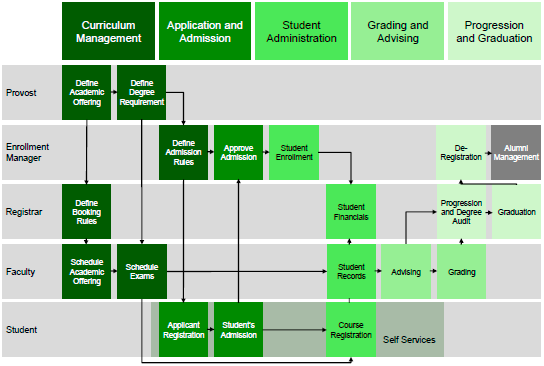
\includegraphics[width=0.8\textwidth]{Materials/Figures/1.png}
    \caption{SAP AG framework of SLM~cite{}}
  \label{SAP}
\end{figure}

%
% ---- Bibliography ----
%
\begin{thebibliography}{99}
%
\bibitem {sap}
Solution in Detail: Higher Education and Research. Student Life Management.
SAP AG, \texttt{http://www.sap.com/bin/sapcom/en\_us/downloadasset.2013-12-dec\newline-11-11.higher-education-and-research-student-lifecycle-\newline management-pdf.html}(2013)

%%%%%%%%%%%%%%%%%%%%%%%%%%%%%%%%%%%%%%%%%%%%%%%%%%%%%%%%%%%%%%%%%%%
\end{thebibliography}
\end{document}             % End of document. 